
\begin{frame}{Componentes EditText y Button en Android}

\textbf{EditText: Campo de Entrada de Texto}
\begin{itemize}
    \item Permite al usuario introducir y editar texto dentro de la aplicación.
    \item Se utiliza en formularios, búsquedas y captura de datos.
    \item Soporta distintos tipos de entrada (texto, número, correo, contraseña).
    \item Puede configurarse mediante atributos XML o código Java/Kotlin.
\end{itemize}

\vspace{0.4cm}

\textbf{Button: Botón de Interacción}
\begin{itemize}
    \item Es un componente que permite al usuario ejecutar acciones al hacer clic.
    \item Se utiliza para enviar datos, navegar entre pantallas o activar eventos.
    \item Puede personalizarse en texto, color, tamaño y estilo.
\end{itemize}


\end{frame}



\begin{frame}[fragile]
\frametitle{Demo 02: Agregar un EditText y un Button}
\begin{columns}
\column{0.80\linewidth}
De los códigos fuentes en Github (como un archivo .zip), descomprimirlo y localizar los archivos mencionados a continuación:
\begin{itemize}
\item Copiar el archivo \textit{MainActivity\_Demo02.java} (dentro del Folder códigosJAVA) al mismo directorio donde esta el \textit{MainActivity.java}.
\item Copiar el archivo \textit{activity\_main\_demo02.xml} (dentro del Folder Carpeta\_layout) al mismo directorio donde esta el \textit{activity\_main.xml}.
\item Modificar en el archivo \textit{AndroidManifest.xml} la cadena \textit{..MainActivity\_Demo01} por \textit{.MainActivity\_Demo02}
\end{itemize}

\begin{block}{Demo \#02}
Muestra una App con dos TextViews, un EditText y un Botton. Cuando el usuario ingresa un dato y presiona le boton aparece un mensaje con el dato ingresado 
\end{block}


\column{0.20\linewidth}

\begin{center}
 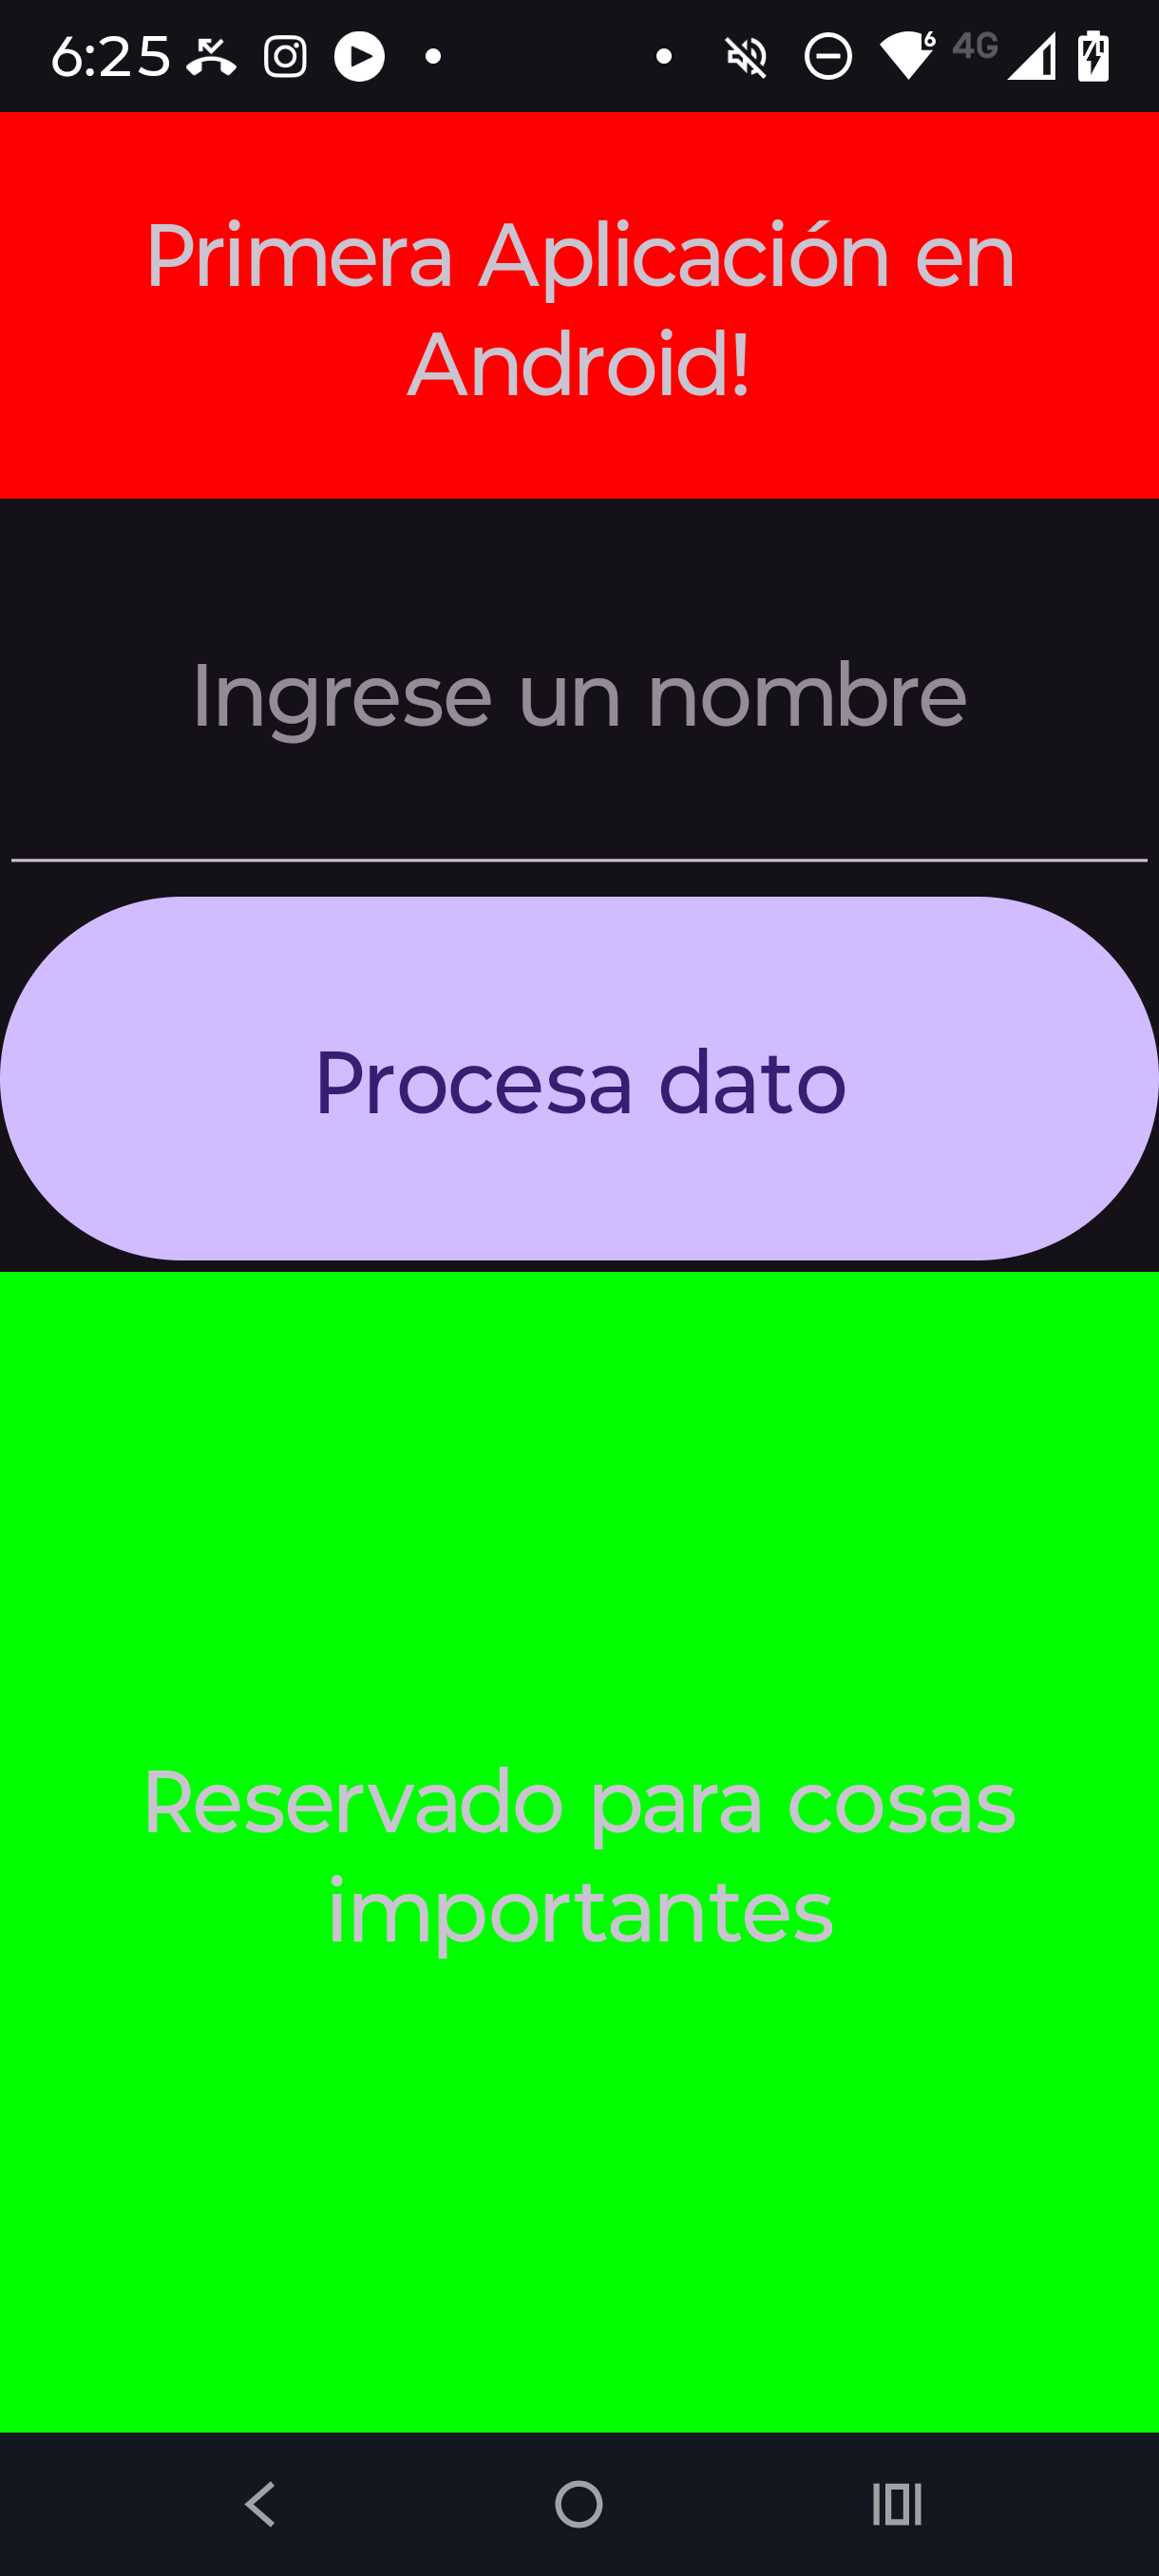
\includegraphics[width=0.98\textwidth]{02_TallerCBTis/figs/Demo02}
\end{center}

\end{columns}

\end{frame}

